%%%%%%%%%%%%%%%%%%%%%%%%%%%%%%%%%%%%%%%%%%%%%%%%%%%%%%%%%%%%%%%%%%%%%%%%%%%%%%%%%%
\begin{frame}[fragile]\frametitle{}
\begin{center}
{\Large Introduction to LangChain}
\end{center}
\end{frame}

%%%%%%%%%%%%%%%%%%%%%%%%%%%%%%%%%%%%%%%%%%%%%%%%%%%%%%%%%%%%%%%%%%%%%%%%%%%%%%%%%%
\begin{frame}\frametitle{What is LangChain?}

Framework built to help you build LLM-powered applications more easily by providing 

\begin{itemize}
\item a generic interface to a variety of different foundation models,
\item a framework to help you manage your prompts 
\item a central interface to long-term memory , external data , other LLMs , and other agents for tasks an LLM is not able to handle (e.g., calculations or search).
\end{itemize}

It is an open-source project (https://github.com/hwchase17/langchain) created by Harrison Chase.

{\tiny (Ref: Getting Started with LangChain: A Beginner’s Guide to Building LLM-Powered Applications by Leonie Monigatti)}
\end{frame}


%%%%%%%%%%%%%%%%%%%%%%%%%%%%%%%%%%%%%%%%%%%%%%%%%%%%%%%%%%%%%%%%%%%%%%%%%%%%%%%%%%
\begin{frame}\frametitle{What is LangChain?}

\begin{itemize}
\item LangChain Open source platform to be used to work with Large Language Models (LLMs). 
\item Integrates will many popular LLM providers like OpenAI, Cohere, Huggingface, and more.  
\item It is designed based on following principles:
	\begin{itemize}
	\item Be Data Aware: connect a language model to other sources of data
	\item Be Agentic: allow a language model to interact with its environment
	\end{itemize}
\item Currently it is available as python and javascript libraries
\item A project initiated by Harrison Chase, but now has rapidly growing contributor and user base (16.1k stars, 367 contributors, 2k forks \& used by 1.6k as of writing this post)!
\end{itemize}

{\tiny (Ref: Linkedin Post by Munjal Patel)}
\end{frame}

%%%%%%%%%%%%%%%%%%%%%%%%%%%%%%%%%%%%%%%%%%%%%%%%%%%%%%%%%%%%%%%%%%%%%%%%%%%%%%%%%%
\begin{frame}\frametitle{What is LangChain?}

\begin{itemize}
\item LangChain can be used to work with Large Language Models (LLMs). 
\item To answer questions about a specific field, like medicine or law. 
\item Popular framework for fine tuning with custom corpus.
\item Gives additional support like meory for chat history etc
\item Chain various LLMs and external apps like Google Search etc.
\end{itemize}

\begin{center}
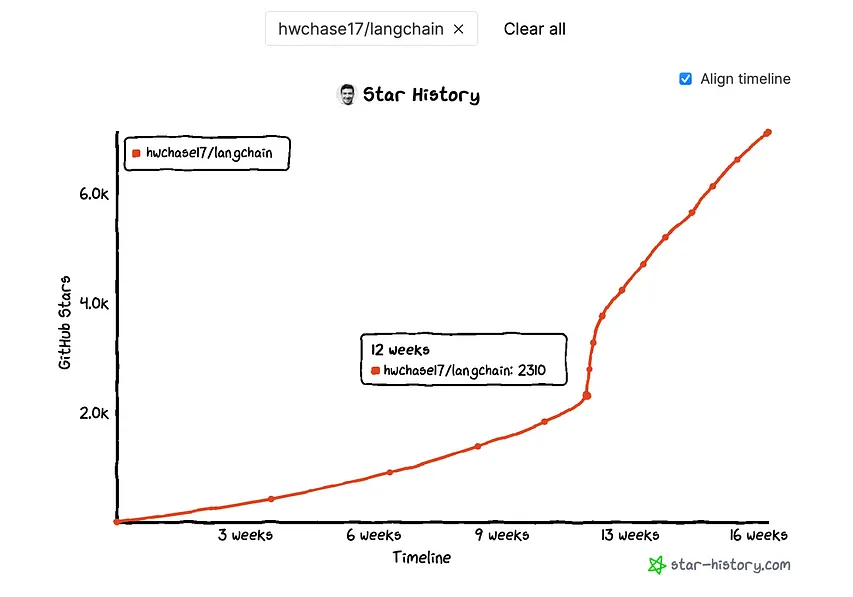
\includegraphics[width=0.6\linewidth,keepaspectratio]{langchain3}
\end{center}	  


{\tiny (Ref: Getting started with LangChain - Avra)}
\end{frame}


%%%%%%%%%%%%%%%%%%%%%%%%%%%%%%%%%%%%%%%%%%%%%%%%%%%%%%%%%%%%%%%%%%%%%%%%%%%%%%%%%%
\begin{frame}[fragile]\frametitle{Setup}

\begin{itemize}
\item Before installing the langchain package, ensure you have a Python version of $> 3.8.1$ and $<4.0$.
\item \lstinline|pip install langchain|
\item Use it as \lstinline|import langchain|
\item LLMs requires API keys for some services you want to use, and some APIs have associated costs.
\item Open-source models: BLOOM by BigScience, LLaMA by Meta AI, Flan-T5 by Google,GPT-J by Eleuther AI, etc
\item Vector Database (optional):  Pinecone, Weaviate, or Milvus etc
\item Tools (optional): OpenWeatherMap or SerpAPI etc
\end{itemize}

{\tiny (Ref: Getting Started with LangChain: A Beginner’s Guide to Building LLM-Powered Applications by Leonie Monigatti)}

\end{frame}

%%%%%%%%%%%%%%%%%%%%%%%%%%%%%%%%%%%%%%%%%%%%%%%%%%%%%%%%%%%%%%%%%%%%%%%%%%%%%%%%%%
\begin{frame}[fragile]\frametitle{What can you do with LangChain?}

\begin{itemize}
\item Models: Choosing from different LLMs and embedding models
\item Prompts: Managing LLM inputs
\item Chains: Combining LLMs with other components
\item Indexes: Accessing external data
\item Memory: Remembering previous conversations
\item Agents: Accessing other tools
\end{itemize}

{\tiny (Ref: Getting Started with LangChain: A Beginner’s Guide to Building LLM-Powered Applications by Leonie Monigatti)}

\end{frame}

%%%%%%%%%%%%%%%%%%%%%%%%%%%%%%%%%%%%%%%%%%%%%%%%%%%%%%%%%%%%%%%%%%%%%%%%%%%%%%%%%%
\begin{frame}[fragile]\frametitle{What can you do with LangChain?}

\begin{itemize}
\item Models: Choosing from different LLMs and embedding models
\item Prompts: Managing LLM inputs
\item Chains: Combining LLMs with other components
\item Indexes: Accessing external data
\item Memory: Remembering previous conversations
\item Agents: Accessing other tools
\end{itemize}

{\tiny (Ref: Getting Started with LangChain: A Beginner’s Guide to Building LLM-Powered Applications by Leonie Monigatti)}

\end{frame}


%%%%%%%%%%%%%%%%%%%%%%%%%%%%%%%%%%%%%%%%%%%%%%%%%%%%%%%%%%%%%%%%%%%%%%%%%%%%%%%%%%
\begin{frame}[fragile]\frametitle{Models: Choosing from different LLMs and embedding models}

LangChain offers integrations to a wide range of models and a streamlined interface to all of them. LangChain differentiates between three types of models that differ in their inputs and outputs:

\begin{itemize}
\item LLMs take a string as an input (prompt) and output a string (completion).
\item Chat models are similar to LLMs. They take a list of chat messages as input and return a chat message.
\item Text embedding models take text input and return a list of floats (embeddings), for calculating similarities between texts (e.g., movie summaries).
\end{itemize}

\end{frame}

%%%%%%%%%%%%%%%%%%%%%%%%%%%%%%%%%%%%%%%%%%%%%%%%%%%%%%%%%%%%%%%%%%%%%%%%%%%%%%%%%%
\begin{frame}[fragile]\frametitle{Hugging Face: Choosing from different LLMs and embedding models}

\begin{lstlisting}
from langchain import HuggingFaceHub
llm = HuggingFaceHub(repo_id = "google/flan-t5-xl")

# The LLM takes a prompt as an input and outputs a completion
prompt = "Alice has a parrot. What animal is Alice's pet?"
completion = llm(prompt)

from langchain.embeddings import HuggingFaceEmbeddings
embeddings = HuggingFaceEmbeddings(model_name = "sentence-transformers/all-MiniLM-L6-v2")

# The embeddings model takes a text as an input and outputs a list of floats
text = "Alice has a parrot. What animal is Alice's pet?"
text_embedding = embeddings.embed_query(text)


\end{lstlisting}


\end{frame}

%%%%%%%%%%%%%%%%%%%%%%%%%%%%%%%%%%%%%%%%%%%%%%%%%%%%%%%%%%%%%%%%%%%%%%%%%%%%%%%%%%
\begin{frame}[fragile]\frametitle{Gen AI Google: Choosing from different LLMs and embedding models}

Prerequisites
\begin{itemize}
\item Select or create a Google Cloud project.
\item Make sure that billing is enabled for your project.
\item Enable the Vertex AI API
\item Create credentials json (Ref https://www.youtube.com/watch?v=rWcLDax-VmM)
\item Set Environment variable GOOGLE\_APPLICATION\_CREDENTIALS as the above created json
\item Create conda environment with \lstinline|python=3.10 (?)|
\item Activating that environment, \lstinline|pip install google-cloud-aiplatform==1.27|
\item Install langchain
\end{itemize}


\end{frame}


%%%%%%%%%%%%%%%%%%%%%%%%%%%%%%%%%%%%%%%%%%%%%%%%%%%%%%%%%%%%%%%%%%%%%%%%%%%%%%%%%%
\begin{frame}[fragile]\frametitle{Gen AI Google: Choosing from different LLMs and embedding models}

Ref https://python.langchain.com/docs/modules/model\_io/models/llms/integrations/google\_vertex\_ai\_palm

\begin{lstlisting}

from langchain.llms import VertexAI
from langchain import PromptTemplate, LLMChain

template = """Question: {question}
Answer: Let's think step by step."""

prompt = PromptTemplate(template=template, input_variables=["question"])
llm = VertexAI()
llm_chain = LLMChain(prompt=prompt, llm=llm)
question = "What NFL team won the Super Bowl in the year Justin Beiber was born?"
response = llm_chain.run(question)
print(response)

llm = VertexAI(model_name="code-bison")
llm_chain = LLMChain(prompt=prompt, llm=llm)
question = "Write a python function that identifies if the number is a prime number?"
response = llm_chain.run(question)
print(response)
\end{lstlisting}


\end{frame}




%%%%%%%%%%%%%%%%%%%%%%%%%%%%%%%%%%%%%%%%%%%%%%%%%%%%%%%%%%%%%%%%%%%%%%%%%%%%%%%%%%
\begin{frame}\frametitle{Why LangChain?}

\begin{itemize}
\item LLMs and Prompts: Prompt management, Prompt optimization, Generic interface for all LLMs and Common utilities for working with LLMs. Powers the agent.
\item Chains: Chains are sequences of calls that whether to an LLM or a different utility. LangChain provides a standard interface for chains, many integrations with other tools, \& end-to-end chains for common applications. Chains go in order.
\item External Data Augmentation: Specific types of chains that first interact with an external data source to fetch data to use in the generation step. Examples of this include summarization of long pieces of text \& question/answering over specific data sources
\item Agents: Agents involve an LLM making decisions about which actions to take, taking that action, seeing an observation, \& repeating that until done. LangChain provides a standard interface for agents, a selection of agents to choose from, and examples of end-to-end agents. Agents decide the next action based on LLM response. Agents are entities that drive decision-making in LangChain. They have access to a suite of tools and can decide which tool to call based on user input. 
\end{itemize}

{\tiny (Ref: Linkedin Post by Munjal Patel)}
\end{frame}


%%%%%%%%%%%%%%%%%%%%%%%%%%%%%%%%%%%%%%%%%%%%%%%%%%%%%%%%%%%%%%%%%%%%%%%%%%%%%%%%%%
\begin{frame}\frametitle{Why LangChain?}

\begin{itemize}
\item Toolkits are sets of tools that, when used together, can accomplish a specific task. The Agent Executor is responsible for running agents with the appropriate tools.
\item Tool: A function that performs a specific duty. This can be things like: Google Search, Database lookup,
\item Memory: Memory refers to the concept of persisting state between calls of a chain/agent. LangChain provides a standard interface for memory, a collection of memory implementations, and examples of chains/agents that use memory.
\item Evaluation [BETA]: Generative models are notoriously hard to evaluate with traditional metrics. One new way of evaluating them is using language models themselves to do the evaluation. LangChain provides some prompts/chains for assisting in this.
\end{itemize}

{\tiny (Ref: Linkedin Post by Munjal Patel)}
\end{frame}


%%%%%%%%%%%%%%%%%%%%%%%%%%%%%%%%%%%%%%%%%%%%%%%%%%%%%%%%%%%%%%%%%%%%%%%%%%%%%%%%%%
\begin{frame}[fragile]\frametitle{Clarifications}

\begin{itemize}
\item A chain is a sequence of components (or other chains) put together to accomplish a specific task. For example, a chain might include a prompt template, a language model, and an output parser, all working together to handle user input, generate a response, and process the output.
\item Chains vs Agents: Whereas a chain defines an immediate input/output process, the logic of agents allows a step-by-step thought process. The advantage of this step-by-step process is that the LLM can work through multiple reasoning steps or tools to produce a better answer.
\item Generic chains as standalone chains are used rarely. There are specialized chains, comprised of many LLMs to help solve a specific task. For example, LangChain supports some end-to-end chains (such as AnalyzeDocumentChain for summarization, QnA, etc) and some specific ones (such as GraphQnAChain for creating, querying, and saving graphs). 
\item Chains can be composed of entities other than LLMs, say, chaining agents and LLMs together.
\end{itemize}

{\tiny (Ref: 'Superpower LLMs with Conversational Agents', 'A Gentle Intro to Chaining LLMs, Agents, and utils via LangChain', etc)}
\end{frame}

%%%%%%%%%%%%%%%%%%%%%%%%%%%%%%%%%%%%%%%%%%%%%%%%%%%%%%%%%%%%%%%%%%%%%%%%%%%%%%%%%%
\begin{frame}[fragile]\frametitle{Clarifications}

\begin{itemize}
\item An agent has access to an LLM to parse the input query and decide the tool to be used and a suite of tools for example Google Search, Python REPL, math calculator, weather APIs, etc. to do the actual work.
\item What’s the point of getting an agent to do the same thing that an LLM can do. Some applications will require not just a predetermined chain of calls to LLMs/other tools, but potentially an unknown chain that depends on the user’s input. In these types of chains, there is an 'agent' which has access to a suite of tools e.g. an agent that can fetch the correct documents (from the vectorstores) for RetrievalQAChain depending on whether the question refers to document A or document B.
\end{itemize}

{\tiny (Ref: 'Superpower LLMs with Conversational Agents', 'A Gentle Intro to Chaining LLMs, Agents, and utils via LangChain', etc)}
\end{frame}

%%%%%%%%%%%%%%%%%%%%%%%%%%%%%%%%%%%%%%%%%%%%%%%%%%%%%%%%%%%%%%%%%%%%%%%%%%%%%%%%%%
\begin{frame}[fragile]\frametitle{Clarifications}

Combine Agent and Chain in another chain.

\begin{lstlisting}
# Chain1 - solve math problem, get the age
chain_one = agent

# Chain2 - suggest age-appropriate gift
template = """You are a gift recommender. Given a person's age,\n
 it is your job to suggest an appropriate gift for them.

Person Age:
{age}
Suggest gift:"""
prompt_template = PromptTemplate(input_variables=["age"], template=template)
chain_two = LLMChain(llm=llm, prompt=prompt_template) 

from langchain.chains import SimpleSequentialChain

overall_chain = SimpleSequentialChain(
                  chains=[chain_one, chain_two],
                  verbose=True)
				  
question = "If my age is half of my dad's age and he is going to be 60 next year, what is my current age?"
overall_chain.run(question)				  
\end{lstlisting}

\end{frame}


%%%%%%%%%%%%%%%%%%%%%%%%%%%%%%%%%%%%%%%%%%%%%%%%%%%%%%%%%%%%%%%%%%%%%%%%%%%%%%%%%%
\begin{frame}\frametitle{LangChain Usecases}

\begin{itemize}
\item Personal assistants
\item Question answering over database(s)
\item Chatbots
\item Querying tabular data
\item Interacting with APIs
\item Model Evaluation
\end{itemize}


{\tiny (Ref: Linkedin Post by Munjal Patel)}
\end{frame}


%%%%%%%%%%%%%%%%%%%%%%%%%%%%%%%%%%%%%%%%%%%%%%%%%%%%%%%%%%%%%%%%%%%%%%%%%%%%%%%%%%
\begin{frame}\frametitle{How LangChain Works?}

\begin{itemize}
\item Text is preprocessed by breaking it down into chunks or summaries, 
\item embedding them in a vector space, 
\item searching for similar chunks when a question is asked. 
\end{itemize}

\begin{center}
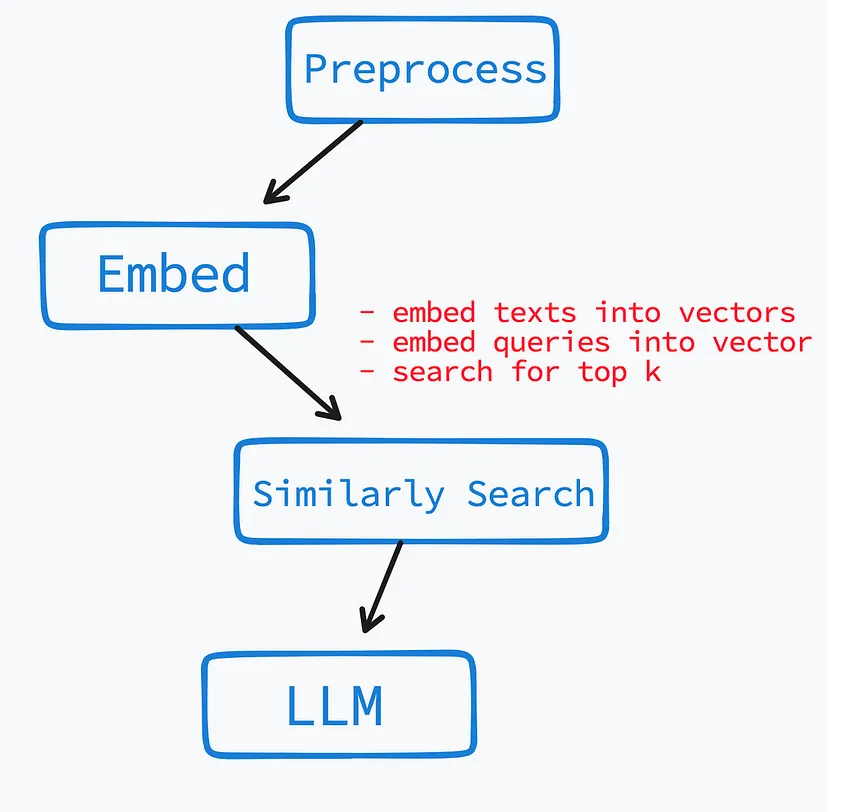
\includegraphics[width=0.5\linewidth,keepaspectratio]{langchain4}
\end{center}	  


{\tiny (Ref: Getting started with LangChain - Avra)}
\end{frame}

%%%%%%%%%%%%%%%%%%%%%%%%%%%%%%%%%%%%%%%%%%%%%%%%%%%%%%%%%%%%%%%%%%%%%%%%%%%%%%%%%%
\begin{frame}[fragile]\frametitle{LangChain Setup}

\begin{lstlisting}
pip install langchain openai cohere huggingface_hub \
ipywidgets chromadb google-search-results

import os
import langchain
from langchain.llms import OpenAI, Cohere, HuggingFaceHub
from langchain.chat_models import ChatOpenAI
from langchain.schema import (
    AIMessage,
    HumanMessage,
    SystemMessage
)
os.environ["OPENAI_API_KEY"] = ""
os.environ["COHERE_API_KEY"] = ""
os.environ["HUGGINGFACEHUB_API_TOKEN"] = ""
os.environ["SERPAPI_API_KEY"] = ""
\end{lstlisting}	  

\end{frame}

%%%%%%%%%%%%%%%%%%%%%%%%%%%%%%%%%%%%%%%%%%%%%%%%%%%%%%%%%%%%%%%%%%%%%%%%%%%%%%%%%%
\begin{frame}[fragile]\frametitle{LangChain Integration}

\begin{lstlisting}
chatgpt = ChatOpenAI(model_name='gpt-3.5-turbo')
gpt3 = OpenAI(model_name='text-davinci-003')
cohere = Cohere(model='command-xlarge')
flan = HuggingFaceHub(repo_id="google/flan-t5-xl")

text = "How to be happy?"

print(chatgpt([HumanMessage(content=text)]))
print(gpt3(text))
print(cohere(text))
print(flan(text))
\end{lstlisting}	  

\end{frame}
